\documentclass{vivid_layout}

% \makeprint is for printing and trimming on paper, w/crop marks.
% \makeprint

%\usepackage{tikz}
%\usetikzlibrary{datavisualization}
%\usetikzlibrary{datavisualization.formats.functions}

%% Required to build cover page
\title{Everything You Need To Know About}{Scalability}
\date{\today}
\cover{scalability/cover}

%% Required to build "Meet the Author"
\author{Baron Schwartz}{img/baron}

%% Required image for "About VividCortex"
\aboutvc{img/presenter}

%% Required resource info
\resourceleft%
	{The Strategic IT Manager's Guide To Building A Scalable DBA Team}
	{}
	{img/scalable-dba-team}
	{https://www.vividcortex.com/resources/building-scalable-dba-team/}
\resourceright%
	{Case Study: SendGrid}
	{VividCortex has been instrumental in finding issues. It's the go-to solution for seeing what's happening in production systems.}
	{img/sendgrid-thumbnail}
	{https://www.vividcortex.com/resources/case-studies/sendgrid/}

\begin{document}
\maketitle		% Build the cover page
\begin{bio}		% Biographical info for "Meet the Author"
Baron is a database expert who is well-known for his contributions to the MySQL, PostgreSQL, and Oracle communities. An engineer by training, Baron has spent his career studying how teams build reliable, high performance systems, and has helped build and optimize database systems for some of the largest Internet properties. Baron has applied his systems thinking skills to both computer systems and teams of people, and has written several books, including O'Reilly's best-selling High Performance MySQL. Prior to founding VividCortex, Baron was an early employee at Percona, where he managed teams including consulting, support, training, and software engineering. Baron has a degree in Computer Science from the University of Virginia.
\end{bio}
\tableofcontents	% Build the table of contents

\section{Introduction}

\section{What is Scalability?}

Scalability is ambiguous for many people---a vague term often tossed about in
conference presentations, for example. It's often used in ways confusingly
similar to performance, efficiency, capacity, availability, and many other terms
related to making things big and fast.

Wikipedia's definition of scalability, borrowed from a 2000 paper by Andr\'e B.
Bondi, is ``Scalability is the capability of a system, network, or process to
handle a growing amount of work, or its potential to be enlarged in order to
accommodate that growth.'' This isn't wrong, but it's still a bit informal, and
this ebook needs a more formal definition.

Dr. Neil J. Gunther provides one such definition: scalability is a {\itshape
function}. I read Dr. Gunther's books and heard him speak for quite a while
before that sunk in for me. Scalability can be defined as a mathematical
function, the relationship between independent and dependent variables (input
and output).

- Most important is getting the x-variable right

Bondi's definition provides a good clue: {\itshape work} is the driving factor
of scalability. Useful ways to think about work include, to mention a few,

\begin{itemize}
\item units of work (requests)
\item the rate of requests over time (arrival rate)
\item the number of units of work in progress at a time (concurrency)
\item the number of customers or users sending requests
\end{itemize}

Each of these can be sensible independent variables for the scalability function
in different circumstances. For example, in benchmarks it's quite common to
configure the number of threads the benchmark uses to send requests to a
database. The benchmark usually sends requests as fast as possible, assuming
zero think time, so the arrival rate is related to, but not strictly controlled
by, the benchmark configuration (since it is determined by how quickly the database finishes each request).

One might say that load or concurrency is the input to the benchmark's
scalability function, and the completion rate is the output.

In another scenario, you might vary the number of CPUs for the system under test
(SUT) while holding constant the load per CPU, or if it's a clustered database,
vary the cluster size and hold constant the load per node. In this case, the
independent variable is the system resources.

In most cases I've analyzed, either concurrency or resources are usually
sensible independent variables for a scalability function.\footnote{I have seen
other scenarios, such as
\href{https://www.percona.com/blog/2011/02/28/is-voltdb-really-as-scalable-as-they-claim/}{scaling
by number of shards}, but we don't need to dig into that in this book.} So for
the purposes of this book, we'll consider scalability to be {\itshape a function
of concurrency or capacity}. The dependent variable is usually the rate at which
the system can process work, or {\itshape throughput}.

XXX chart with axes

For those who are like me and need extra emphasis, I'll repeat that this is a
mathematical function, with concurrency or capacity on the $X$ axis, and
throughput on the $Y$ axis.

\section{Linear Scalability: The Holy Grail}

In my experience, never was a marketechture slide deck created that mentions
scalability without also including the word "linear." But like many other things
in scalability, that word is {\itshape horribly} abused.

XXX PRINCESS BRIDE MEME

Hand-waving claims of linear scaling usually coincide with vague definitions
of scalability, and people who know a lot about scalability rarely say the word
``linear.'' Here are a few of the misdefinitions of linear scalability I've heard:

\begin{itemize}
\item A web architect at a conference said, ``I designed our system to be
shared-nothing so it would be linearly scalable.'' He meant there was no
single resource or system imposing a hard upper limit on how many servers could
be added to the system. But he didn't really know whether his system actually
scaled linearly.
\item A technical evangelist giving a presentation about a clustered database
said, ``adding a node to the cluster adds a predictable amount of capacity.''
Predictable isn't the same as linear.
\item A sales presentation for another clustered database said the database
``scales linearly, with a linearity factor of 97\%,'' meaning that each
additional node increases the system's capacity by 0.97 times the amount the
previous node added. That's a curve, not a line.  (Later you'll learn how to
instantly determine the asymptotic upper bound on such a system's total
capacity.)
\end{itemize}

This may seem like a pointless rant, but it's actually important if you want to
be able to design and improve highly scalable systems.

Spotting bogus linearity claims is fun. Here are some ways
to make systems appear linear:

\begin{itemize}
\item Show graphs without numbers, so you can't do the math.
\item Show graphs with nonlinear axes.
\item Begin the axes, especially the $Y$ axis, at a nonzero value.
\end{itemize}

Here is an example that employs some of these tricks.
\begin{center}
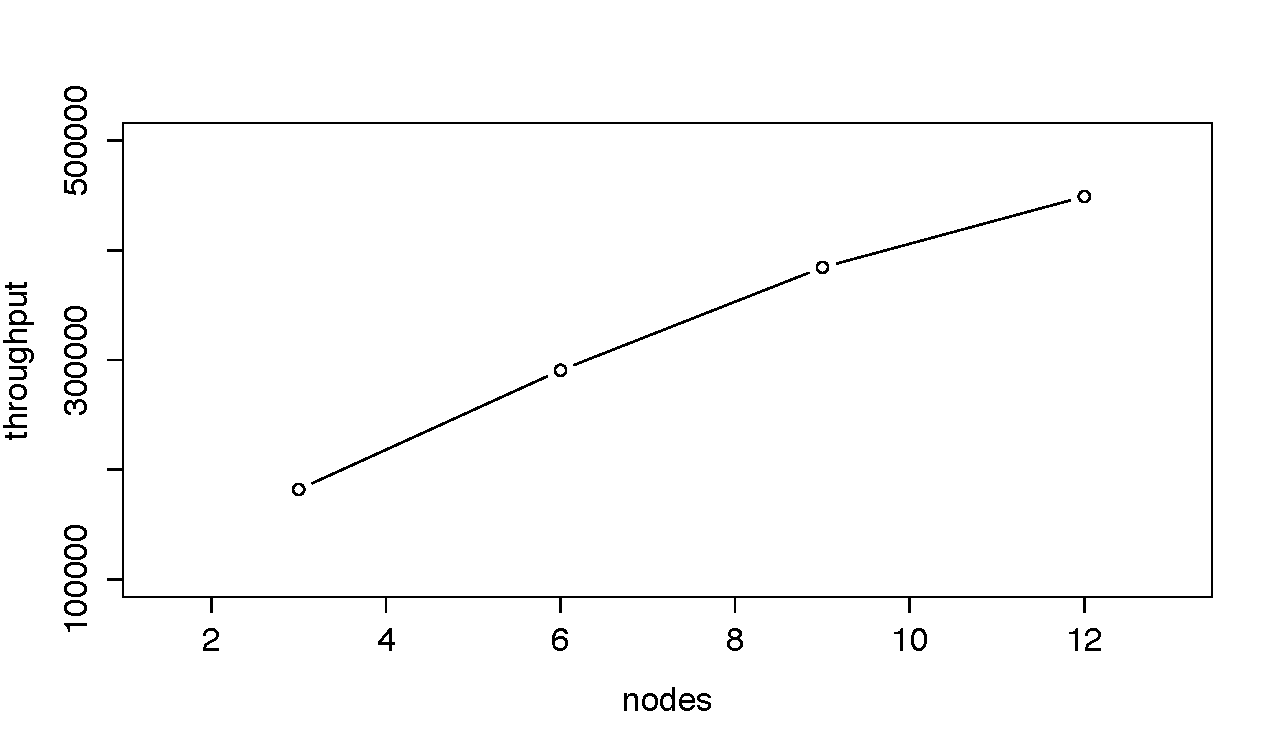
\includegraphics[width=.85\linewidth]{scalability/voltdb1}
\end{center}
Looks pretty linear, doesn't it? Yet if you do the math, it's nowhere near
linear.  It's an optical illusion, because the $X$ axis begins around
1.45 instead of zero, and the $Y$ axis starts at 100000, so you can't tell that
the chart isn't going to intersect the origin if you extend it downwards.

{\bfseries The real test of linearity is whether the transactions per second per
node remains constant as the node count increases}. The chart's original source
mentioned that throughput increased from ``182k transactions per second for 3
nodes to 449k for 12 nodes.'' The math is easy: the system achieves 60700
transactions per second per node at 3 nodes, but only 37400 at 12 nodes, which
represents a {\itshape 39\% drop in throughput} versus linear scalability.  If
it actually scaled linearly, it would achieve 728k transactions per second at 12
nodes.

Linear means linear, folks! And seemingly small amounts of nonlinearity really
matter, as you'll see later, because small sublinear effects grow very quickly
at larger scale.\footnote{In fact, they grow---wait for it---nonlinearly!}

\section{Why Systems Scale Sublinearly}

Linear scalability is the ideal, yet despite the claims, systems that actually
scale linearly are rare.  It's very useful to understand the reasons for this,
because a correct understanding of scalability, and the reasons and sources of
sublinear scaling, is the key to building more scalable systems.  That's why
it's really important to be a linearity skeptic.  It's not just being pedantic.

The best way to think about linearity is as a ratio of the system's performance
at a size of 1, if possible. Neil Gunther calls this the {\itshape efficiency}.
If a system produces 1800 transactions per second with 1 node, then ideally 4
nodes produce 7200 transactions per second. That would be 100\% efficient. If
the system loses a bit of efficiency with each node and 4 nodes produce, say,
5180 TPS, the system is only 72\% efficient:
\begin{center}
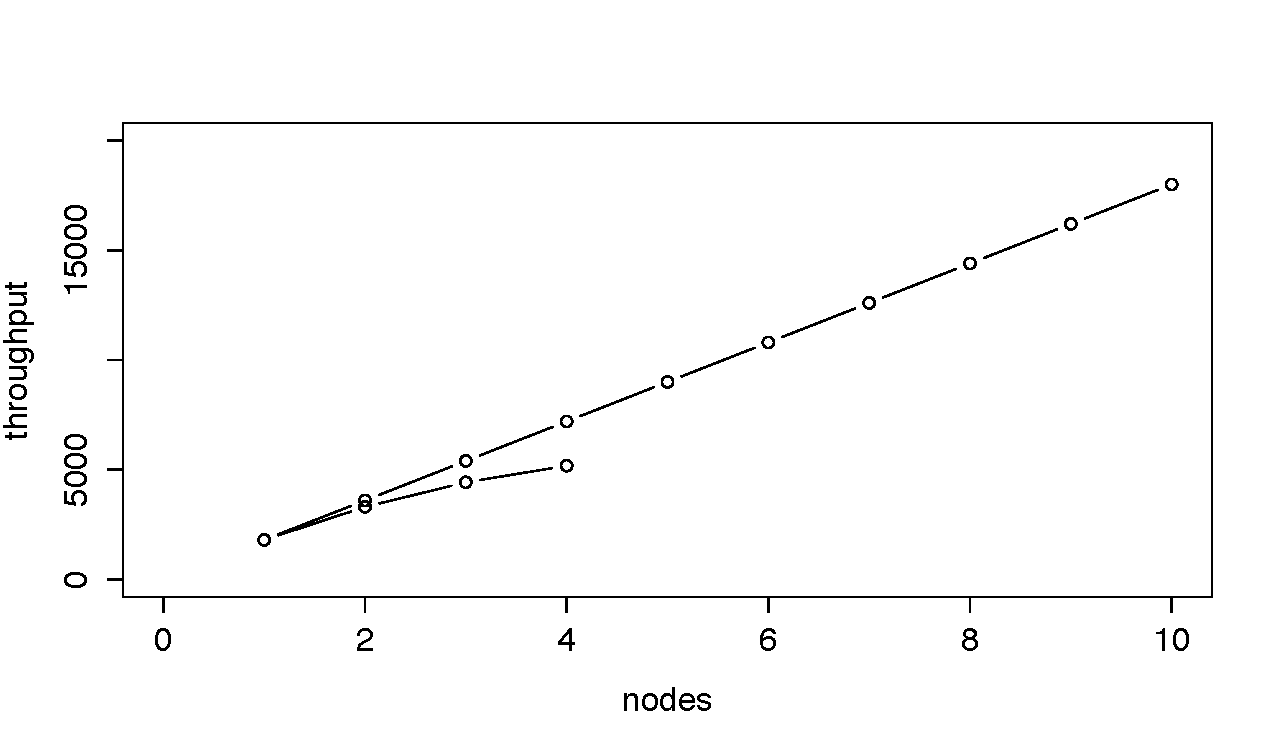
\includegraphics[width=.85\linewidth]{scalability/linear2}
\end{center}
If you do this math, you'll often be surprised at how large the loss of
efficiency is.  Graphs can be deceptive, but the numbers are quite clear.
\footnote{Drawing a linear scaling line on the graph helps, too. Without that
line, the eye tends to see the graph as more linear than it really is, and the
loss of efficiency becomes less obvious.}


In the real world there's almost always some loss of efficiency, and if you can
figure out why, you may be able to fix it. In fact, you've probably noticed that
real systems tend not only to fall behind linear scalability a bit, but actually
exhibit {\itshape retrograde} scalability at some point:
\begin{center}
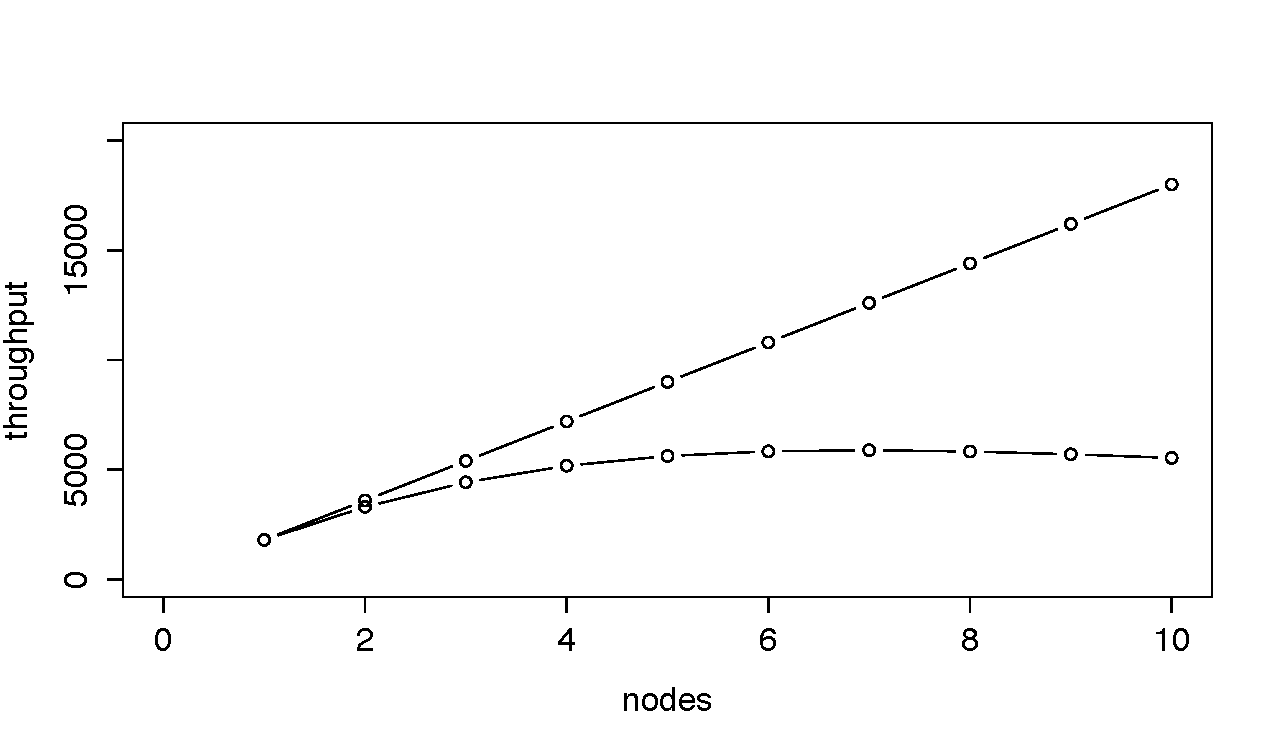
\includegraphics[width=.85\linewidth]{scalability/linear3}
\end{center}
This is quite common in the real world---you scale things up and at some point
your system starts going backwards and {\itshape losing} performance, instead of
just gaining more and more slowly. In the MySQL 5.0 days, for example, it was
common to see people getting better performance out of 4-core servers than
8-core servers.

Why does this happen? Why don't systems scale linearly, and why do they
sometimes show retrograde scalability?

According to Dr. Gunther, there are two reasons: {\bfseries serialization} and
{\bfseries crosstalk}. Serialization degrades scalability because parts of the
work can't be parallelized, so speedup is limited. Crosstalk introduces a
fast-growing coherency delay as workers (threads, CPUs, etc) block on shared
mutable state and communication mechanisms. We'll explore these effects in the
next section.

\section{The Universal Scalability Law}

Dr. Neil J. Gunther's Universal Scalability Law (USL) provides a formal
definition of scalability,\footnote{Gunther originally called the USL
``superserial,'' and you may encounter this terminology, especially in older
books and papers.} and a conceptual framework for understanding,
evaluating, comparing, and improving scalability. It does this by quantifying
the effects of linear speedup, serialization delay, and coherency delay due to
crosstalk.

Let's see how this works, piece by piece. An ideal system of size 1
achieves some amount $\lambda$ of throughput $X$, in completed requests per
second. Because the system is ideal, the throughput doubles at size $N$=2, and so
on. This is perfect linear scaling:
\[
X(N) = \frac{\lambda N}{1}
\]

The $\lambda$ parameter defines the slope of the line. I call it the {\itshape
coefficient of performance}. It's how fast the system performs in the special
case when there's no serialization or crosstalk penalty.  Note that every
linearly scalable system is just as scalable as any other, regardless of the
slope of the line. They have different performance but identical scalability
characteristics: speedup is unlimited. Here are two ideal systems, with
$\lambda$ of 1800 and 800, respectively.
\begin{center}
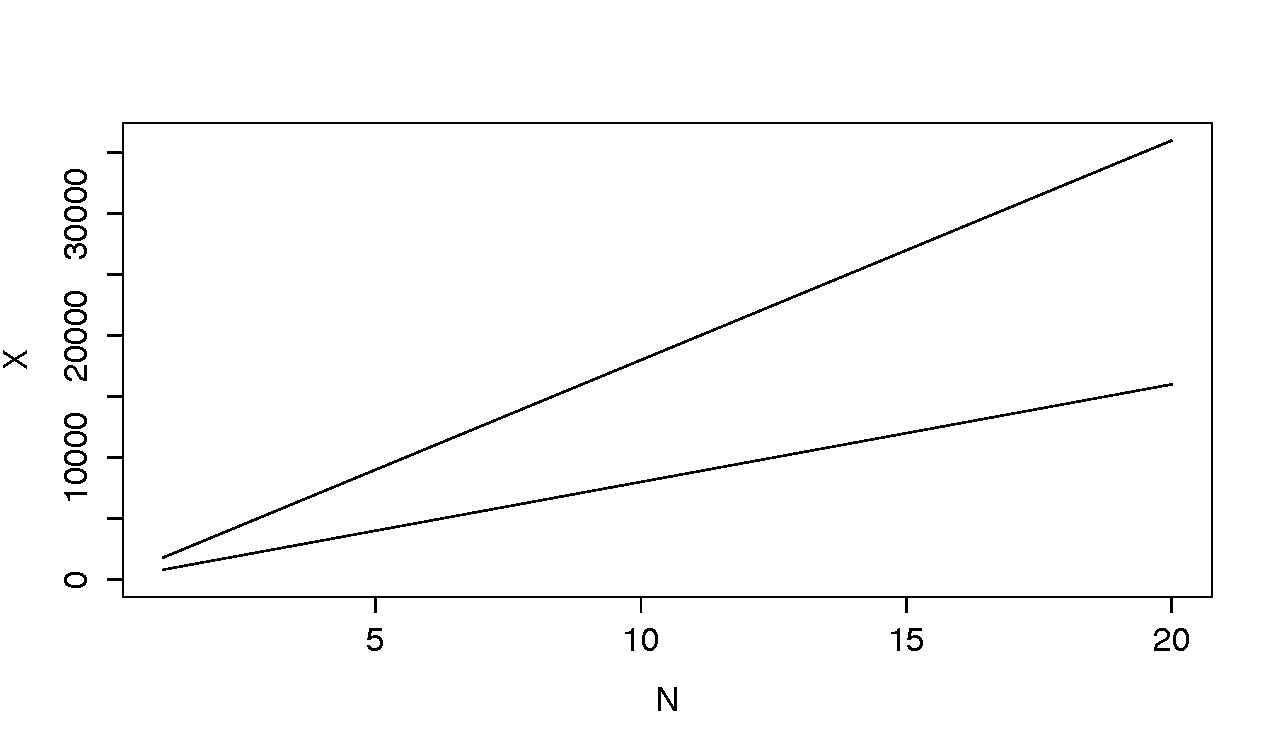
\includegraphics[width=.85\linewidth]{scalability/ideal-linear}
\end{center}

Serialization appears in most human and computer systems at some point, for
example as a final stage of assembling the multiple outputs generated in
parallel into a single final result. As parallelization increases, serialization
becomes the limiting factor. This is codified in
\href{https://en.wikipedia.org/wiki/Amdahl\%27s\_law}{Amdahl's Law}, which states that
the maximum speedup possible is the reciprocal of the serial fraction. This fits
neatly into the bottom of the equation. Here $\sigma$ is the serial fraction of
the work, the {\itshape coefficient of serialization}:
\[
X(N) = \frac{\lambda N}{1 + \sigma(N-1)}
\]

The resulting system will asymptotically approach a ceiling on speedup. If
$\sigma$ is .05, for example, the speedup approaches 20.
\begin{center}
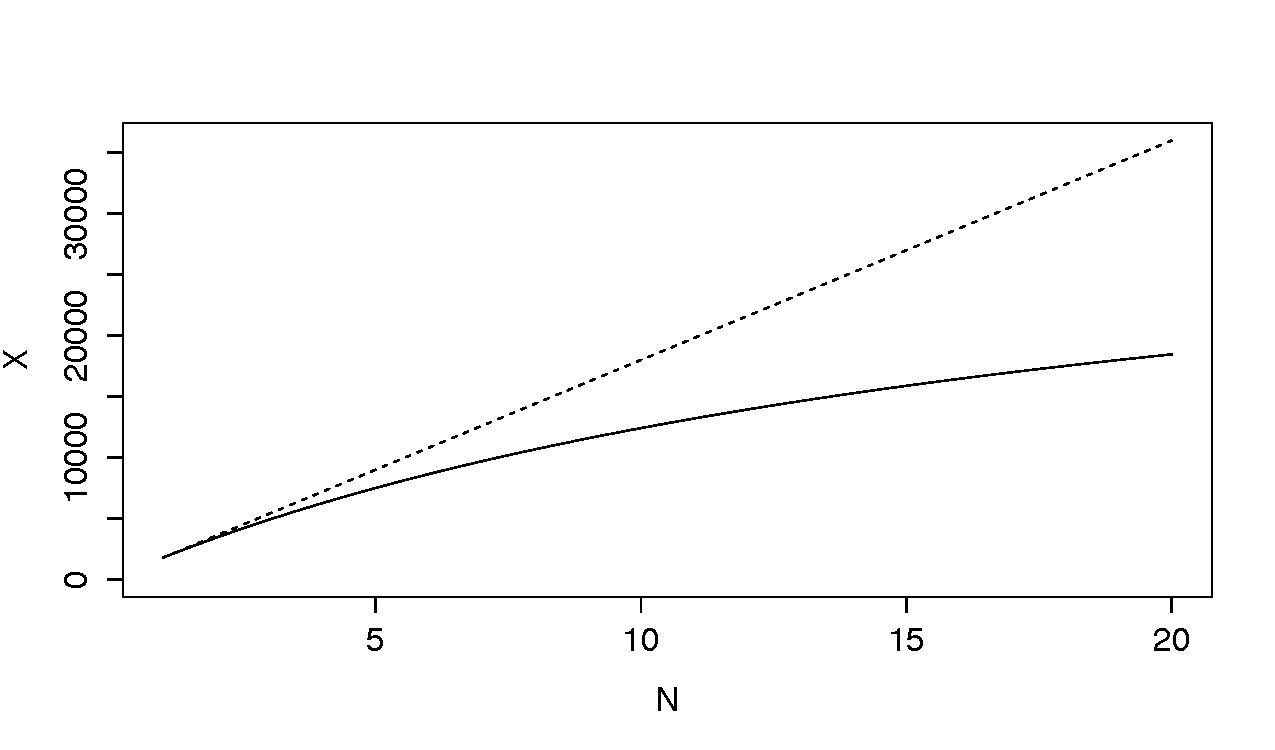
\includegraphics[width=.85\linewidth]{scalability/amdahl}
\end{center}

The last bit is the crosstalk penalty. Crosstalk potentially happens between
each pair of workers in the system (threads, CPUs, servers, etc). We represent the amount of crosstalk with another parameter, $\kappa$.

You probably remember that the number of edges in a fully connected graph is
$n(n-1)$, which is on the order of $n^2$ in the long run.\footnote{If you're
not familiar with it,
\href{https://www.vividcortex.com/blog/2013/10/23/big-o-notation-made-simple/}{this
blog post introduces Big-O notation}.} The $\kappa$ coefficient quantifies the
crosstalk in the denominator:
\[
X(N) = \frac{\lambda N}{1 + \sigma(N-1) + \kappa N(N-1)}
\]

The crosstalk penalty grows fast. Because it's quadratic, eventually it grows
faster than the linear speedup of the ideal system we started with, no matter
how small $\kappa$ is.  That's what makes retrograde scalability happen:
\begin{center}
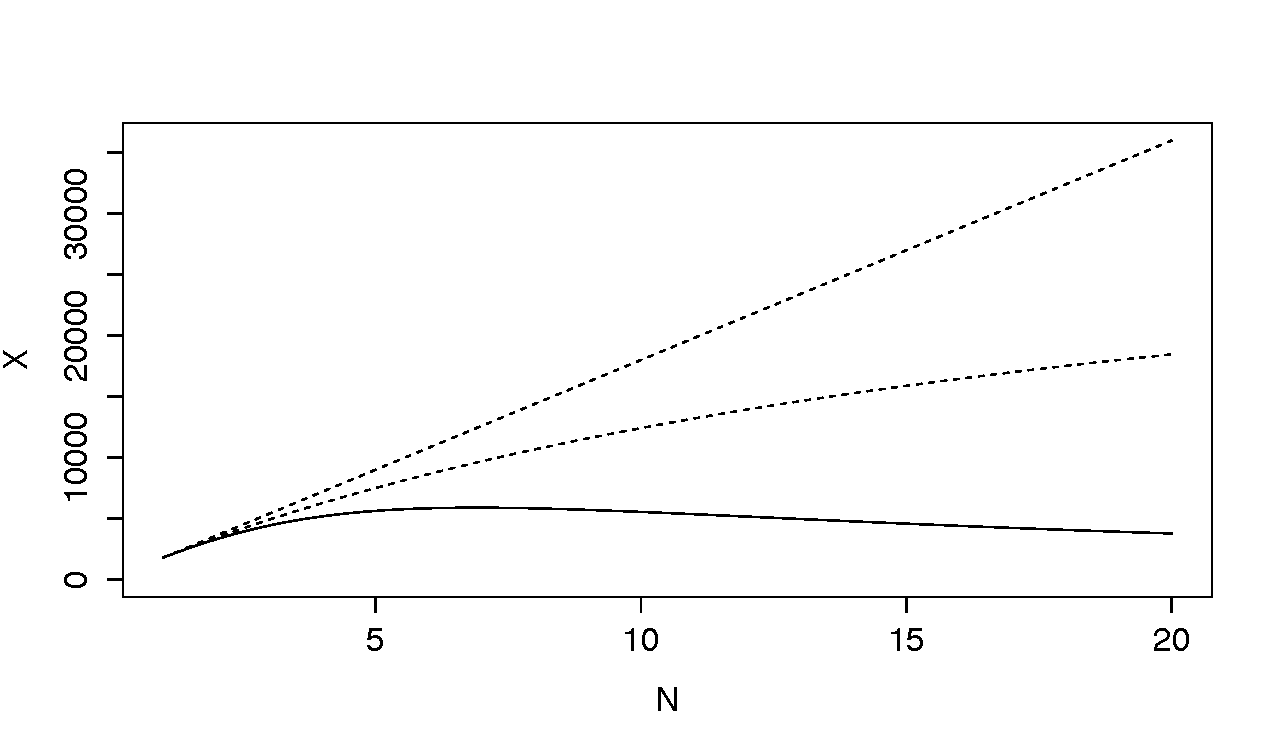
\includegraphics[width=.85\linewidth]{scalability/usl}
\end{center}

That's the Universal Scalability Law in all its glory.  This plot has the same
parameters as the ones I showed before, where a system of size 4 produced only
72\% of its ideal output. That system has 5\% serialization and 2\% crosstalk,
and now that I've plotted it out to size 20 you can see it's embarrassingly
inefficient.  In fact, we should have given up trying to scale this system after
size 6 or so.

This shows visually how much harm a ``small amount'' of nonlinearity can do in
the long run.  Even very small amounts of these damaging coefficients will
create this effect sooner or later (mostly sooner). This is why it's rare to
find clustered systems that scale well beyond a couple dozen nodes or so.
If you'd like to experiment with this interactively, I've made a graph of it at
\href{https://www.desmos.com/calculator/2l0jcjmsxn}{Desmos}.

If you're curious, the USL is based on queueing theory. It's equivalent to
synchronous repairman queueing. You can read more about that in Neil Gunther's
books. If you're not familiar with queueing theory, I wrote a highly
approachable introduction called
\href{https://www.vividcortex.com/resources/queueing-theory/}{Everything You
Need To Know About Queueing Theory}.

\section{Measuring Scalability}

To recap, up until now we've figured out the right dimensions for a formal model
of scalability that seems to behave as we know real systems behave, and examined
Neil Gunther's USL, which fits that framework well and gives us an equation for
scalability. (Are you excited yet?)

Now what do we do with it?

Great question! It turns out we can do a lot of extremely useful things with it.
Unlike a lot of models of system behavior, this one is actually practical to
apply in the real world. That's the real genius of it, in fact. Not only is the
equation uncomplicated, but the variables it describes are easy to get from a
lot of systems.  If you've ever tried to model system behavior with queueing
theory, e.g. the Erlang C formula, you're going to love how simple it is to get
results with the USL. So many modeling techniques are foiled by the inability to
get the measurements you need.

The thing I've used the USL for the most is measuring system scalability, by
working backwards from observed system behavior and deriving the likely
coefficients. To accomplish this, you need a set of measurements of the system's
size as you see fit to define it (usually concurrency or node count) and
throughput. Then you {\itshape fit} the USL to this dataset, using nonlinear
least squares regression. This is a statistical technique that finds the optimal
coefficient values in order to calculate a best-fit line through the
measurements. The result is values for $\lambda$, $\sigma$, and $\kappa$.

If you're reading about the USL in Neil Gunther's books, he takes a different
approach. First, he doesn't use regression to determine $\lambda$, he assumes
that is something you can measure in a controlled way at $N=1$. (I've often
found that's not true for me.) Secondly, there are a couple of different forms
of the USL---one for hardware scaling and one for software scaling---which are
the same equation, but with different parameters. I've found the distinction to
be largely academic, although I will talk a bit more about this later.

Examples of systems I've analyzed with the USL include:

\begin{itemize}
\item Black-box analysis of networked software simply by observing and
correlating packet arrivals and departures, looking at the IP addresses, port
numbers, and timestamps. From this I computed the concurrency by averaging the
amount of time the system was busy servicing requests over periods of time. The
throughput was straightforward to get by counting packet departures.
\item MySQL database servers. Some of its \texttt{SHOW STATUS} counters are
essentially equivalent to throughput and concurrency.
\item Linux block devices (disks) by looking at \texttt{/proc/diskstats}, from
which you can get both instantaneous and average concurrency over time deltas,
as well as throughput (number of I/Os completed).
\item Lots and lots---and lots---of benchmark results.
\end{itemize}

I've built a variety of tools to help clean, resample, and analyze the data
before arriving at satisfactory results. Most of them were commandline, though
these days I use R more than anything else. This is an important topic, though I
don't have time to go into it in detail: you will get dirty data, and that will
make your results useless. You need to visualize both in scatterplot form as
well as in time-series form and ensure you're working with a relatively
consistent set of data. You can remove individual points or trim the time range
you use, and you may need to experiment with averaging the data over time to get
good results.

As for the R code, I'll give a little bit of a quickstart to show the
soup-to-nuts approach.  You'll save the data into a delimited file, with column
headers \texttt{size} and \texttt{tput}. Then you'll load this into a variable
in R and regress it against the USL.

Here's a complete sample, based on a
\href{https://www.percona.com/docs/wiki/benchmark:cisco:scale:start}{benchmark}
that Vadim Tkachenko ran at Percona:

\begin{verbatim}
size tput
1 955.16
2 1878.91
3 2688.01
4 3548.68
5 4315.54
6 5130.43
7 5931.37
8 6531.08
9 7219.8
10 7867.61
11 8278.71
12 8646.7
13 9047.84
14 9426.55
15 9645.37
16 9897.24
17 10097.6
18 10240.5
19 10532.39
20 10798.52
21 11151.43
22 11518.63
23 11806
24 12089.37
25 12075.41
26 12177.29
27 12211.41
28 12158.93
29 12155.27
30 12118.04
31 12140.4
32 12074.39
\end{verbatim}

Save that data into a file, say, \texttt{benchmark.txt}. Then load it and run the following commands:

\begin{verbatim}
benchmark <- read.csv("/path/to/benchmark.txt", sep="")
usl <- nls(tput ~ lambda*size/(1 + sigma * (size-1) + kappa * size *
   (size-1)), benchmark, start=c(sigma=0.1, kappa=0.01, lambda=1000))
summary(usl)
sigma <- coef(usl)['sigma']
kappa <- coeff(usl)['kappa']
lambda <- coef(usl)['lambda']
u=function(x){y=x*lambda/(1+sigma*(x-1)+kappa*x*(x-1))}
plot(u, 0, max(benchmark$size)*2, xlab="Size", ylab="Throughput", lty="dashed")
points(benchmark$size, benchmark$tput)
\end{verbatim}

The results are as follows:
\[
\begin{array}{ll}
			\lambda&995.6486 \\
     \sigma & 0.02671591 \\
			       \kappa & 0.0007690945 \\
\end{array}
\]

Note the extremely small value for $\kappa$ which nonetheless degrades
scalability before $N$ becomes very large. Here's the resulting plot:
\begin{center}
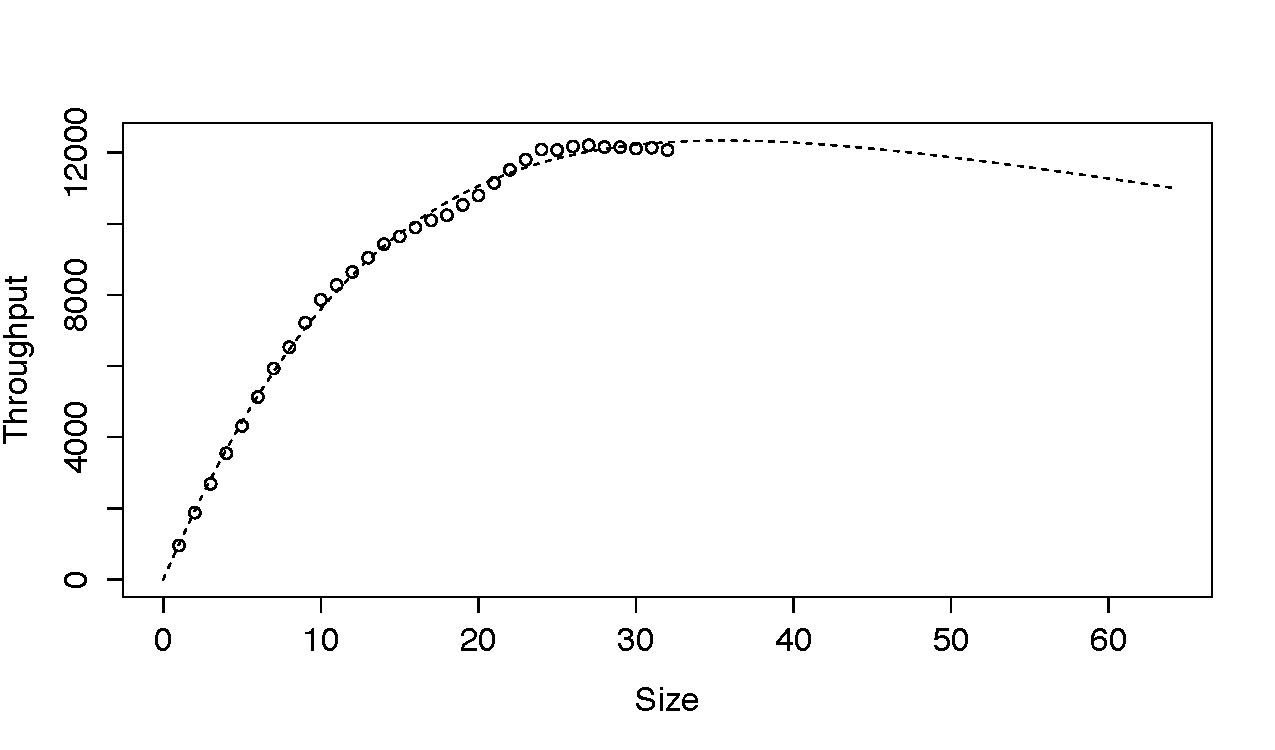
\includegraphics[width=.85\linewidth]{scalability/cisco}
\end{center}

If you're an R user, that's probably all you need to get going. You really
should do more diligence, such as checking the $R^2$ value of the fit. But
instead of doing all this work manually (which you can certainly do if you
want), I suggest using the
\href{https://cran.r-project.org/web/packages/usl/}{USL package from CRAN}. It
has all the niceties built in.

One final thing: if the $kappa$ coefficient has a nonzero value, the function
has a maximum. You can find the size of the system at that maximum as follows:
\[
N_{max} = \left \lfloor \sqrt{\frac{1-\sigma}{\kappa}} \right \rfloor
\]

Of course, to find the maximum predicted throughput, you just plug $N_{max}$
into the USL equation itself. Doing so with the coefficients in this example
predicts the system's throughput will increase until $N=35$, which in this case
means 35 threads, and the peak throughput will be 12341 queries per second. It
also found $lambda$, the throughput at $N=1$, to be 995 QPS, which is close to
the actual value of 955.

It's always interesting to use the USL on a subset of the performance data, such
as the first third or so, to see how well it predicts the higher $N$ values.
This can be quite educational.

Note that you should have at least half a dozen or so data points in order to
get good results in most circumstances. In practice I usually try to capture at
least a dozen for benchmarks, and more---often thousands---when analyzing
systems that aren't in a controlled laboratory setting.

\section{Relating Scalability and Performance}



  request performance is response time
  system performance is throughput
  USL already predicts and explains system performance
  but what about request performance, can we predict it too?
	little's law says yes, we can
	just use it to predict avg response time at a given concurrency
	\[
	y=\frac{1+s(x-1)+kx(x-1)}{c}
	\]
	https://www.desmos.com/calculator/vjlnruxxdi
	is it valid? is r-time quadratic wrt concurrncy? if so then appd might be OK
	don't confuse this with r-time and utilization chart; concur -> infinity
	further reading: neil claims that this is not universally valid
	"Be careful. That's only true when Z = 0 (user/generator think time). 
	Otherwise, you miss the "foot" of the hockey stick."
 * https://groups.google.com/d/topic/guerrilla-capacity-planning/hei8zL2muuE/discussion
  * http://perfdynamics.blogspot.com/2015/07/hockey-elbow-and-other-response-time.html
  however, in my tests of real world systems, it is exactly right
  it does not predict the dsn of resp time, only avg, however you could use
  queueing theory to predict that, given the offered load and thus the rho

\section{Capacity Planning with the USL}
  common question - how much work can I handle with this system?
  - will I need more for the holidays?
  - how much spare runway do I have?
  - hard to tell, often inscrutable whether we're close to a breaking point
  USL's max capacity equation predicts max thruput
  but that's not really max capacity
  capacity  is max work-getting-done with SLA of good perf (typically as percentile)
  at this point, system probably gives horrible perf
	 by he way this is a problem with benchmarks - they push the system bad perf
	 benchmarks are always unrealistic
	predicting system capacity is something queueing theory is often used for
	predict utilization, etc
 * queueing theory - hard because of service times
	  * USL instead; much easier to measure
  - forecasting - lets us predict beyond what we can measure
  - show one of the datasets with only part of the data, does it predict the
  rest?
  - best and worst cases; repairman queueing
  - where is the sublinearity coming from (paypal nodejs)
  - using it to see approx what \% of capacity we're at now
  - see also the queueing theory book and square root staffing

\section{the usl in real life}
  - how well does it work
	The USL is wrong:
	theoretical physicist, Richard Feynman:
	“In general we look for a new law by the following process: first we guess it.
	Don’t laugh -- that’s really true. Then we compute the consequences of the guess
	to see what, if this law is right, what it would imply. Then we compare those
	computation results to nature, i.e. experiment and experience. We compare it
	directly to observation to see if it works.
	“If it disagrees with experiment, it’s wrong. That simple statement is the key
	to science. It doesn’t make a difference how beautiful your guess is, it doesn’t
	make a difference how smart you are, who made the guess or what his name is --
	if it disagrees with experiment, it’s wrong. That’s all there is to it.”
	(Cornell lecture, 1964)

  - 
      * ceilings from hitting something’s max capacity like network tput
		    * usually queueing causes retrograde to grow even faster than
			 predicted
	- note that one could conjecture and analyze other shapes like the USL, e.g.
	https://www.desmos.com/calculator/nl53iwbngn
	\[
	u\left(x\right)=\frac{bx}{1+s\left(x-1\right)+kx\left(x-1\right)}\left\{x>0\right\}
	\]
	\[
	l\left(x\right)=\frac{bx}{1+s\left(x-1\right)+k\ln\left(x\right)\left(x-1\right)}\left\{x>0\right\}
	\]
	\[
	r\left(x\right)=\frac{bx}{1+s\left(x-1\right)+k\sqrt{x}\left(x-1\right)}\left\{x>0\right\}
	\]
	- Jayanta Choudhury has suggested changes to fit better.
\section{superlinear scaling}
	- special cases: aggregate capacity not scaling proportionately to load,
	dataset, etc so each "worker" has some advantage
	- special case: 1 and 2 nodes
	- effect of "economies of scale," that is a resource that is more efficient
	when shared than when used singly
	- https://queue.acm.org/detail.cfm?id=2789974
\section{other PoV on scapability}
	- alternative - quadratic scalability. Impossible because it goes negative.
	It's just wrong. Might as well draw a line with your hand and one of those
	template curves. https://en.wikipedia.org/wiki/French\_curve
	https://www.graphicsdirect.co.uk/french-curve-set.html
	- alternative definitions of scalability - new relic
	 http://www.xaprb.com/blog/2013/01/07/a-close-look-at-new-relics-scalability-chart/

	, appd, riak
	- cockcroft headroom plots
* How to improve scalability
    * avoid crosstalk
	     * avoid serialization
		      * avoid queueing
* Further reading
				    * GCaP
					     * Look at the Percona white paper


Example data
* http://obartunov.livejournal.com/181981.html
  http://www.postgrespro.ru/blog/pgsql/2015/08/30/p8scaling
  scaling/scaling-postgrespro.png
* VoltDB
* mat keep
https://blogs.oracle.com/MySQL/entry/comparing\_innodb\_to\_myisam\_performance
https://www.percona.com/blog/2011/01/26/modeling-innodb-scalability-on-multi-core-servers/
* paypal example
https://www.vividcortex.com/blog/2013/12/09/analysis-of-paypals-node-vs-java-benchmarks/
* example of robert haas
http://rhaas.blogspot.com/2011/09/scalability-in-graphical-form-analyzed.html


\newpage

\begin{about}	% Build "About VividCortex"
VividCortex is a SaaS database performance monitoring. The database is the heart of most applications, but it's also the part that's hardest to scale, manage, and optimize even as it's growing 50\% year over year. VividCortex has developed a suite of unique technologies that significantly eases this pain for the entire IT department. Unlike traditional monitoring, we measure
and analyze the system's work and resource consumption. This leads directly to better performance for IT as a whole, at reduced cost and effort.
\end{about}
\makeresources	% Build "Related Resources"
\end{document}
